%%%%%%%%%%%%%%%%%%%%%%%%%%%%%%%%%%%%%%%%%%%%%%
%                insertmeeting
% 1) Title (something creative & funny?)
% 2) Date (MM/DD/YYYY)
% 3) Location (ex. Hagerty High School)
% 4) People/Committees Present 
% 5) Picture 
% 6) Start Time & Stop Time (ex. 12:30AM to 4:30PM)
%%%%%%%%%%%%%%%%%%%%%%%%%%%%%%%%%%%%%%%%%%%%%%
\insertmeeting 
	{Let's Get Digital} 
	{09/23/21}
	{Hagerty High School}
	{Clayton, Jensen, Nathan, Ritam}
	{Images/RobotPics/robot.jpg}
	{2:30 - 4:30}
	
\subsection*{Software}
\noindent\hfil\rule{\textwidth}{.4pt}\hfil
\subsubsection*{Goals}
\begin{itemize}
    \item Set up Android studio
    \item set up TRC code   
    \item Set up a new Github repository for this years code
    \item Help all new programming team members obtain a github account 
\end{itemize} 

\noindent\hfil\rule{\textwidth}{.4pt}\hfil

\subsubsection*{Accomplishments}
Today, we worked on setting up a 4717 github repository so we can wirelessly communicate between different computers relatively seamlessly. The repository has different folders for CAD and Programming, among others. Each subset has different permissions as to who can access it to prevent accidental changes to our CAD or program. First, we had all the new members create new accounts in GitHub, as shown in Figure \ref{fig:pic1}. Everyone contributes to the repository, as shown in Figure \ref{fig:pic2}. In order to communicate these files from one person to another, knowing how to pull and push files will be necessary, as shown in Figures \ref{fig:pic3} and \ref{fig:pic4}. 
 
We accomplished our goals of setting up Android studio and the TRC code.
 

\begin{figure}[ht]
\centering
\begin{minipage}[b]{.50\textwidth}
  \centering
  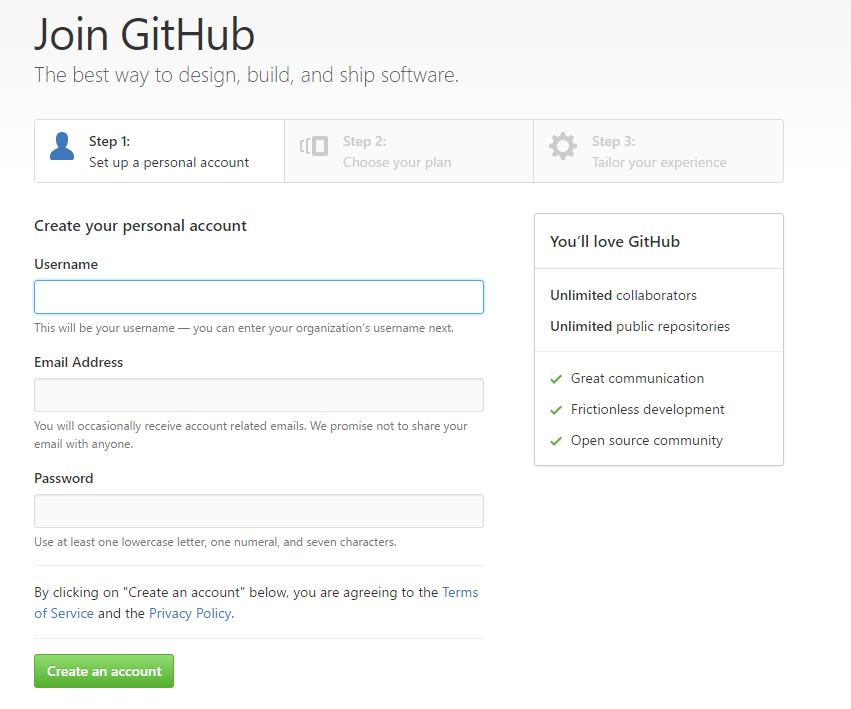
\includegraphics[width=0.5\textwidth]{Meetings/September/09-23-21/githubnewacc.png}
  \caption{New Account in Github}
  \label{fig:pic1}
\end{minipage}%
\hfill%
\begin{minipage}[b]{.50\textwidth}
  \centering
  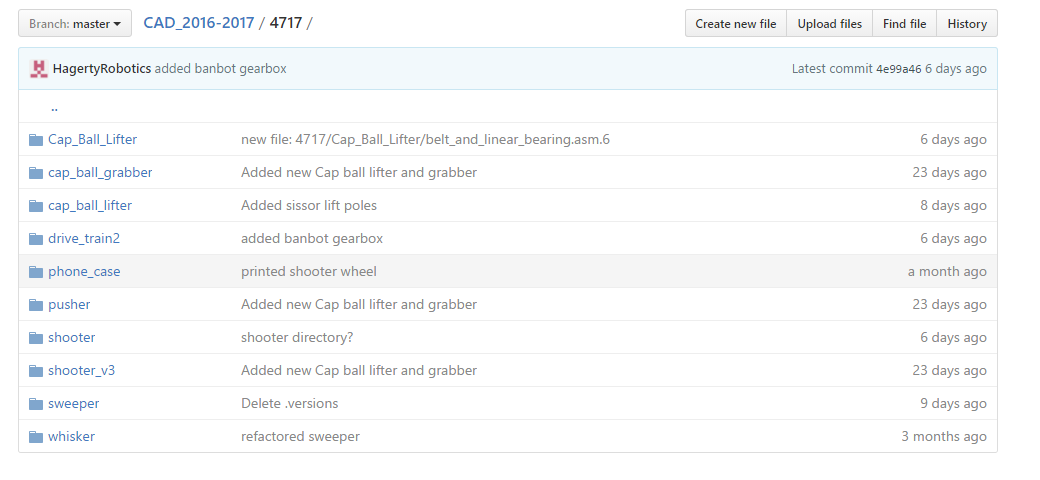
\includegraphics[width=0.8\textwidth]{Meetings/September/09-23-21/githubrepository.png}
  \caption{Screenshot of GitHub Repository}
  \label{fig:pic2}
\end{minipage}
\end{figure}




\begin{figure}
\centering
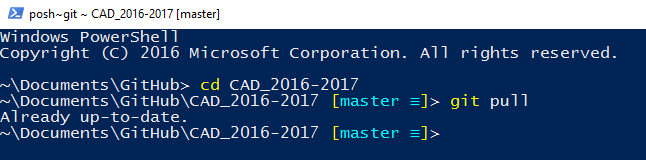
\includegraphics[width=0.85\textwidth, angle=0]{Meetings/September/09-23-21/gitshellpull.png}
\caption{GitShell Pull Files}
\label{fig:pic3}
\end{figure}


\begin{figure}
\centering
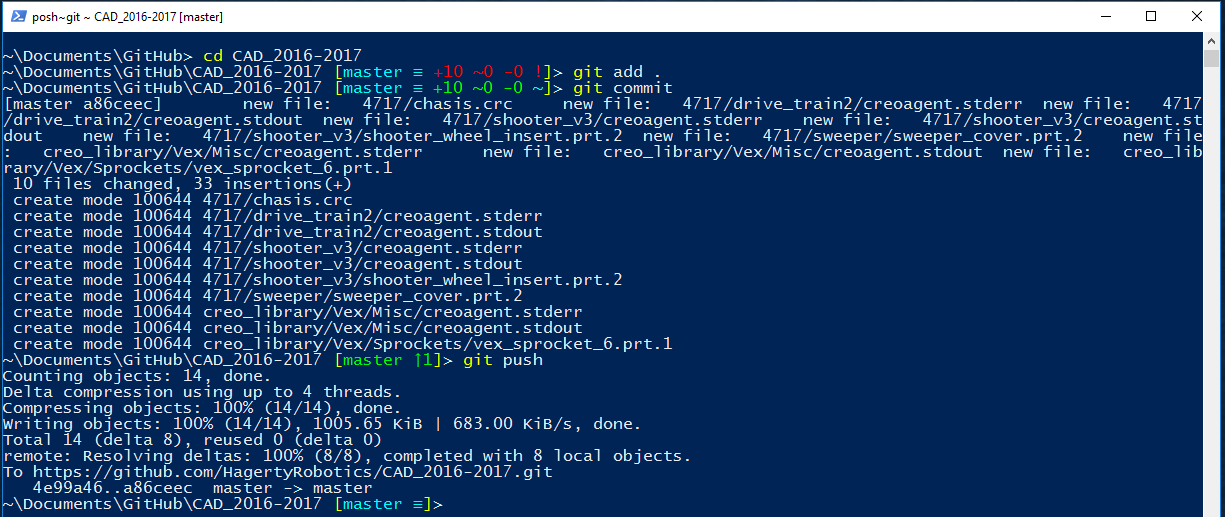
\includegraphics[width=0.85\textwidth, angle=0]{Meetings/September/09-23-21/gitshellpush.png}
\caption{GitShell Push Files}
\label{fig:pic4}
\end{figure}


\subsection*{Hardware}
\noindent\hfil\rule{\textwidth}{.4pt}\hfil
\subsubsection*{Goals}
\begin{itemize}
    \item Discus drivetrain designs
    \item Come up with a plan for prototyping
\end{itemize} 

\noindent\hfil\rule{\textwidth}{.4pt}\hfil

\subsubsection*{Accomplishments}
Today we wanted to tackle the monumental task of designing our drivetrain. Deciding on a design will be our first step in creating our robot, so we all started excitedly talking about the ideas we’ve had since the game reveal on Saturday. One of these ideas was inspired by another team’s drivetrain from a couple years back. The team, Up a Creek robotics (team 11260), designed a very odd but effective drivetrain for their rover ruckus robot. Instead of reaching over the crater like most other teams, they designed their robot like a mars rover so that they could drive over the edge of the crater (Figure \ref{fig:banemod}). The drivetrain looks very reliable, and the crater is much taller than the barriers are this year so the design seems very feasible. Although we considered starting off with this design, we don't want to just copy something someone else made and call it our own. Another concern is that it might be over complicated. The craters from the rover ruckus season were much bigger and more difficult to get over than the 1 inch pipe barriers from this year. 
Instead of using something similar to UP a Creek’s design, we decided to go ahead and test a much simpler tank drive. We plan to make this drivetrain small and light so that we can go over the barriers easily. Although we usually use a tank drive with 4 motors and 6 wheels, this new design will only use 2 motors on the entire drivetrain and will have 4 wheels. The decrease in the amount of motors will make this prototype lighter and having 2 wheels will reduce the risk of the center wheel getting stuck in between the barriers. We got this idea from one of our school’s vex robotics teams who we were talking to a couple days ago. Their base drivetrain is built similarly to how we plan to build ours, using 2 motors and 4 wheels, connected using chains and sprockets. To ensure that this plan was viable, we talked to one of our mentors about the plan. He gave it a thumbs up, but added the suggestion of building the prototype out of the REV parts we just ordered. In addition to being easy to work with rev, parts are pretty light and will be a good prototyping tool for the drivetrain. 

\begin{figure}
\centering
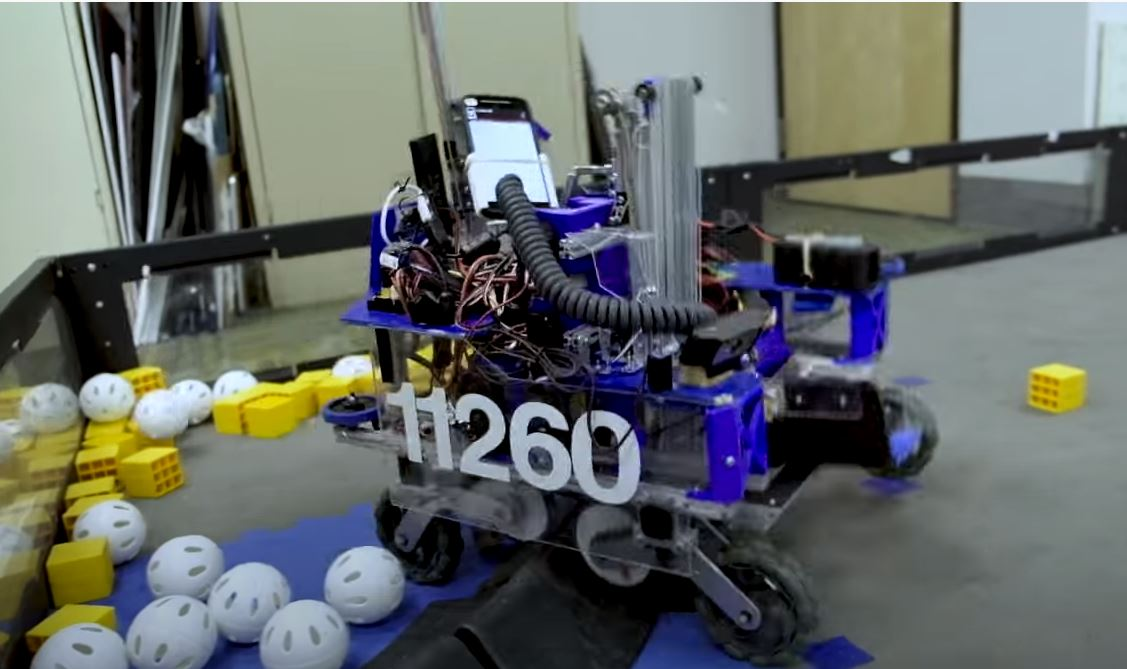
\includegraphics[width=0.85\textwidth, angle=0]{Meetings/September/09-23-21/9-21-21_Hardware_Image1 - Nathan Forrer.JPG}
\caption{11260's drivetrain for Rover Ruckus}
\label{fig:pic4}
\end{figure}





